% One capsule of the packed bed, melting from its surface inwards
\documentclass[tikz, border=4pt]{standalone}
% Shared preamble of the PyTES model diagrams: packages, colours and styles.
% Each diagram is a standalone document that inputs this file; build them with build.py.
\usepackage{amsmath}
\usepackage{bm}
\usetikzlibrary{arrows.meta, calc, decorations.pathreplacing, patterns, positioning}

% The PyTES Thermal colour cycle (pytes.plotting.THERMAL) and tints of it
\definecolor{pytesorange}{HTML}{E8590C}
\definecolor{pytesblue}{HTML}{1F4E9C}
\definecolor{pytesteal}{HTML}{14A08A}
\definecolor{pytesamber}{HTML}{F0A930}
\definecolor{pytesplum}{HTML}{A23B72}
\definecolor{pytessky}{HTML}{88C7F0}
\definecolor{pytesink}{HTML}{36312E}

% Materials: the heat transfer fluid, the PCM, the metal (fins and tubes)
\colorlet{fluidfill}{pytessky!75}
\colorlet{pcmfill}{pytesamber!55}
\colorlet{liquidfill}{pytesorange!60}
\colorlet{metalfill}{pytesink!45}
\colorlet{compositefill}{pcmfill!85!metalfill}

\tikzset{
  >={Stealth[length=2.2mm]},
  every picture/.style={line join=round, line cap=round, font=\small},
  outline/.style={draw=pytesink, line width=0.6pt},
  fluid/.style={outline, fill=fluidfill},
  pcm/.style={outline, fill=pcmfill},
  liquid/.style={outline, fill=liquidfill},
  metal/.style={outline, fill=metalfill},
  composite/.style={outline, fill=compositefill},
  flow/.style={->, draw=pytesblue, line width=1.2pt},
  heat/.style={->, draw=pytesorange, line width=1.1pt},
  axis/.style={->, draw=pytesink, line width=0.7pt},
  dimension/.style={<->, >={Stealth[length=1.6mm]}, draw=pytesink, line width=0.5pt},
  guide/.style={draw=pytesink!60, line width=0.4pt, dashed},
  symmetry/.style={draw=pytesink, line width=0.5pt, dash dot},
  label/.style={text=pytesink, font=\small},
  note/.style={text=pytesink, font=\footnotesize, align=center},
}

\begin{document}
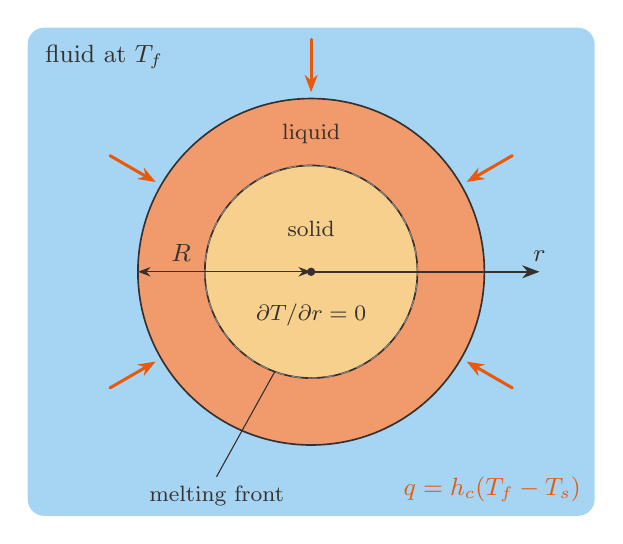
\begin{tikzpicture}
  \def\R{2.2}
  \def\front{1.35}
  % The fluid around the capsule
  \fill[fluidfill, rounded corners=6pt] (-3.6, -3.1) rectangle (3.6, 3.1);
  \node[label, anchor=north west] at (-3.5, 3.0) {fluid at $T_f$};
  % Liquid shell and solid core
  \draw[liquid] (0, 0) circle (\R);
  \draw[pcm] (0, 0) circle (\front);
  \draw[guide] (0, 0) circle (\front);
  \node[note] at (0, 0.55) {solid};
  \node[note] at (0, 1.75) {liquid};
  \draw[pytesink, line width=0.4pt] ({\front*cos(250)}, {\front*sin(250)}) -- (-1.2, -2.6)
    node[note, below] {melting front};
  % Coordinate and radius
  \fill[pytesink] (0, 0) circle (1.5pt);
  \draw[axis] (0, 0) -- (2.9, 0) node[label, above] {$r$};
  \draw[dimension] (0, 0) -- (-\R, 0) node[label, pos=0.75, above] {$R$};
  \node[note] at (0, -0.55) {$\partial T/\partial r = 0$};
  % Heat flux from the fluid through the surface
  \foreach \a in {30, 90, 150, 210, 330} {
    \draw[heat] ({(\R + 0.75)*cos(\a)}, {(\R + 0.75)*sin(\a)})
      -- ({(\R + 0.08)*cos(\a)}, {(\R + 0.08)*sin(\a)});
  }
  \node[label, text=pytesorange, anchor=south east] at (3.55, -3.05)
    {$q = h_c (T_f - T_s)$};
\end{tikzpicture}
\end{document}
